\section{Introduction}

\begin{figure}[H]
    \centering
    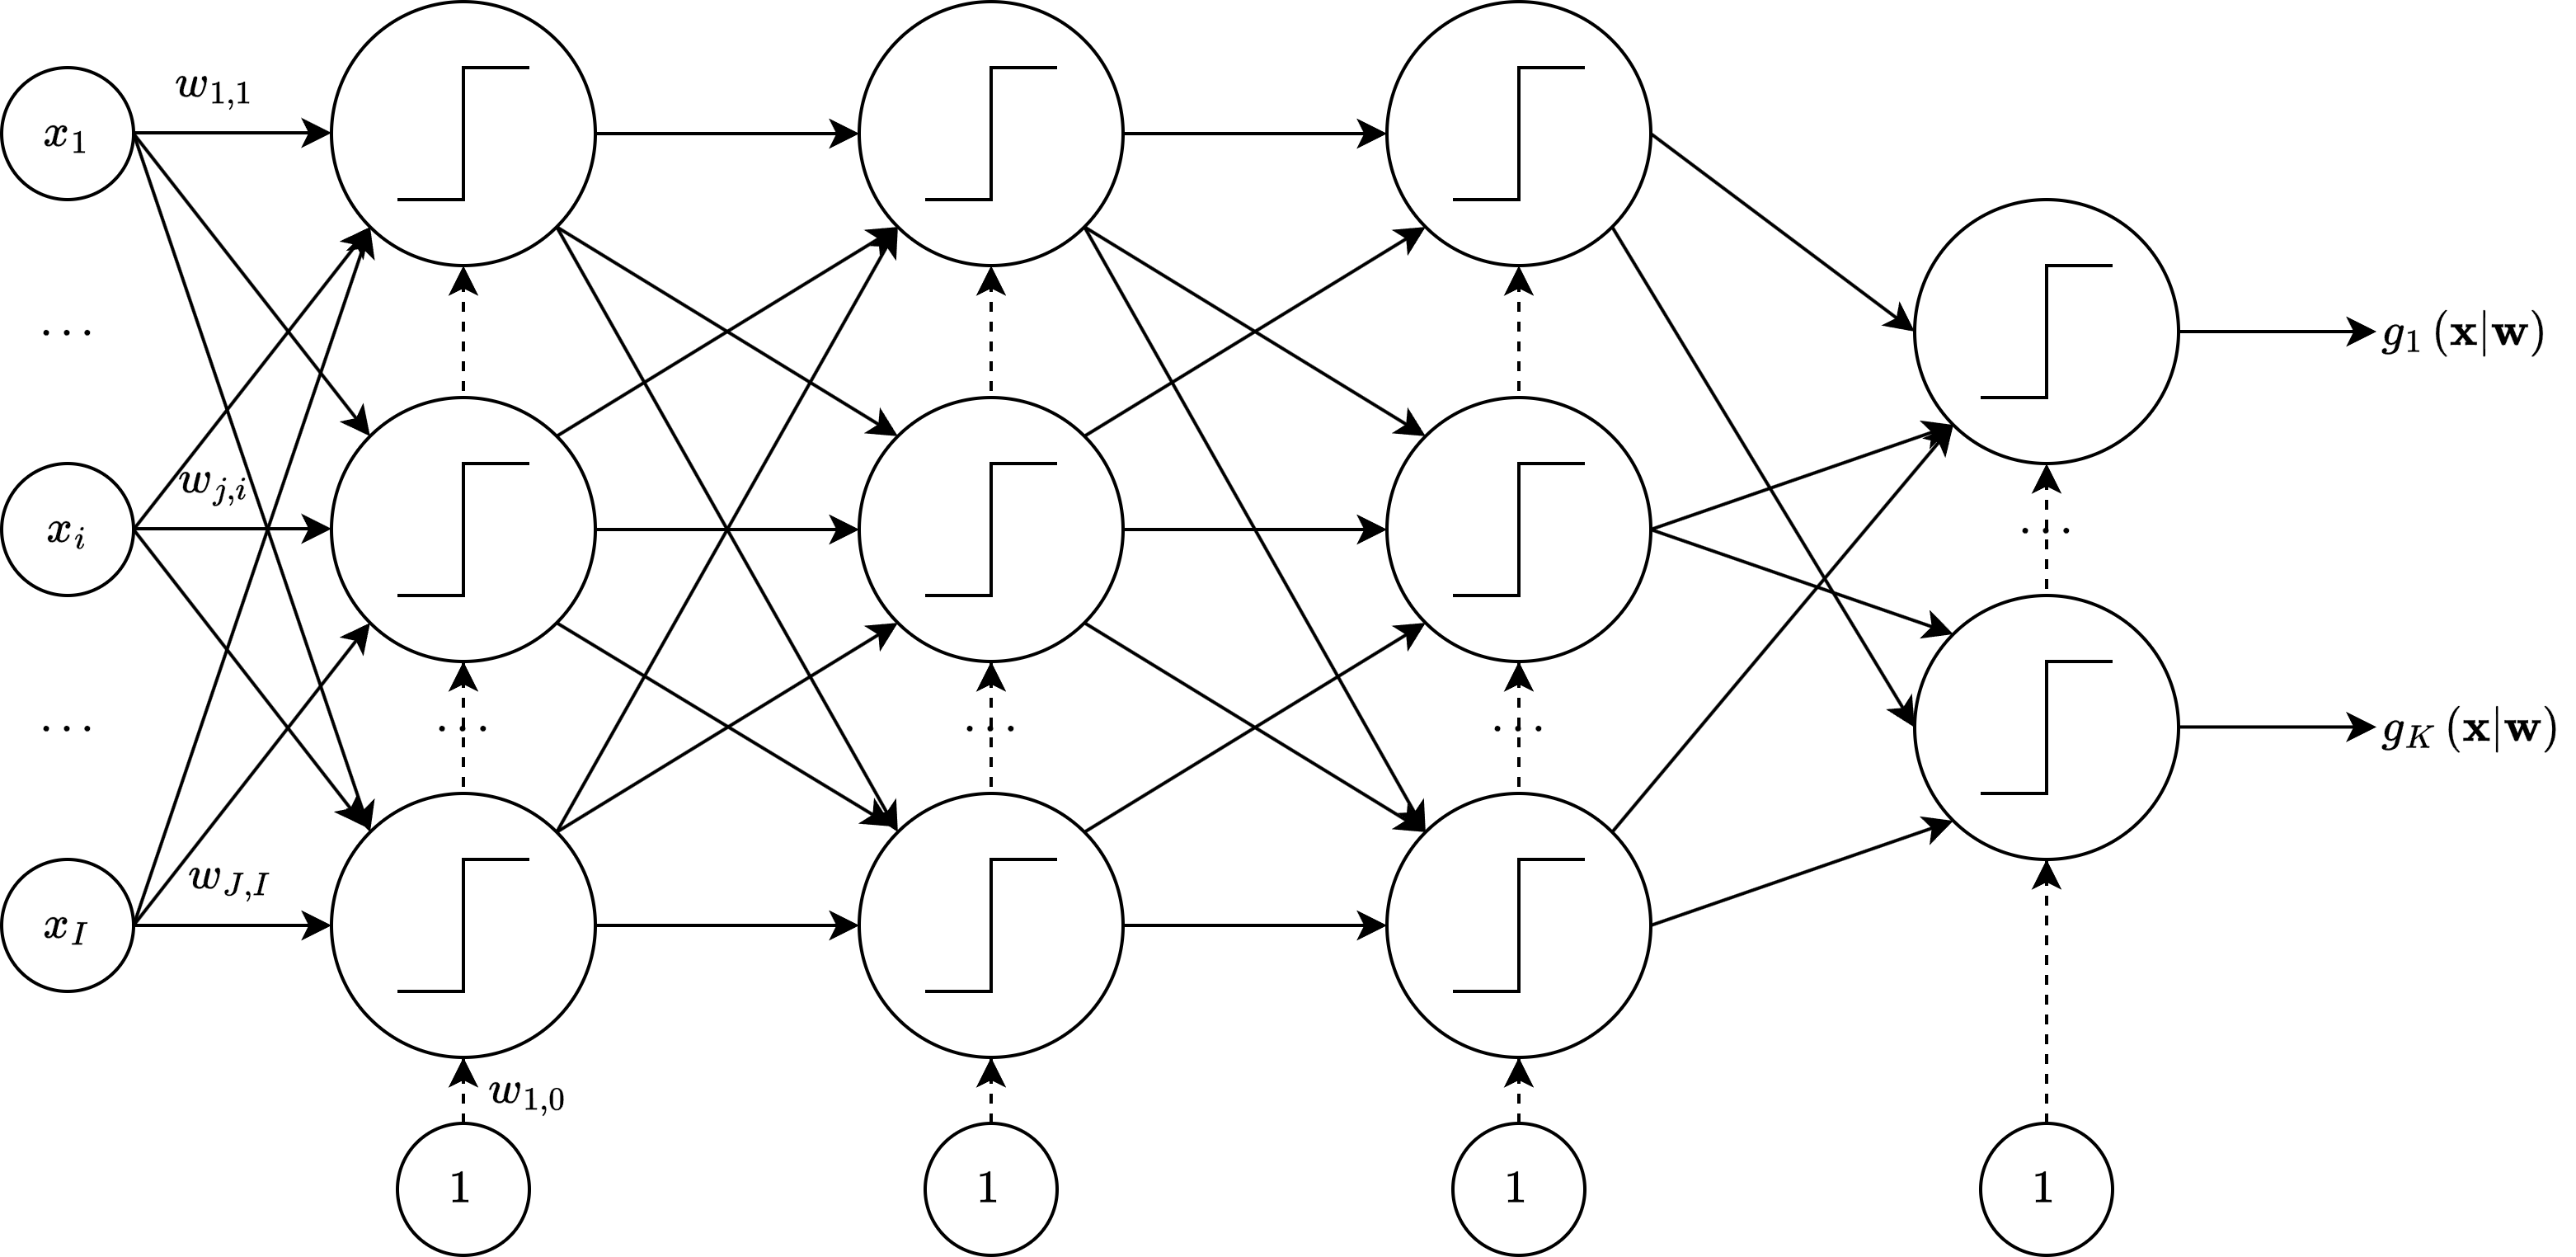
\includegraphics[width=0.75\linewidth]{images/ffnn.png}
    \caption{Multi-Layer Perceptron architecture}
\end{figure}
A Multi-Layer Perceptron (MLP) is a type of feedforward neural network (FFNN) that consists of multiple layers of nodes, each layer being fully connected to the next. 
The MLP architecture is composed of three primary components:
\begin{itemize}
    \item \textit{Input layer}: this layer receives the input data and passes it to the subsequent layers. 
        The size of this layer depends on the specific problem and the input features.
    \item \textit{Hidden layers}: these intermediate layers perform the actual computations, transforming the input into more abstract representations. 
        The number of hidden layers and the number of neurons in each hidden layer are determined through hyperparameter tuning, which is often based on a trial-and-error approach.
    \item \textit{Output layer}: this layer produces the final output of the network, which could be a prediction, classification, or another result. 
        Its size depends on the nature of the problem, such as the number of classes in classification tasks.
\end{itemize}
The MLP is inherently a non-linear model, characterized by the number of neurons in each layer, the choice of activation functions, and the values of the connection weights.
The connections between layers are represented by weight matrices, denoted as $W^{(l)}=\{w_{ij}^{(l)}\}$, where $l$ is the layer index. 
If a layer has $J$ nodes and receives $I$ inputs, the corresponding weight matrix has dimensions $J \times (I+1)$ accounting for the bias term.

The output of each neuron depends solely on the outputs from the previous layer, allowing for forward propagation of information. 
The learning of weights in an FFNN is achieved through a technique known as backpropagation, which iteratively adjusts the weights to minimize the error in the network's predictions.